% !TEX encoding = UTF-8
% !TEX TS-program = pdflatex
% !TEX root = ../tesi.tex

%**************************************************************
\chapter{Performance}
\label{cap:performance}
%**************************************************************
\section{Confronto dei vari metodi}
In questa sezione confronteremo il tempo di esecuzione dei vari metodi risolutivi per 5 configurazioni iniziali del problema, di difficoltà crescente dal livello 0 al livello 4.\\
Per i primi 4 problemi abbiamo anche un dato del tempo impiegato da una persona nel risolvere il problema. Abbiamo infatti sottoposto i vari livelli a 8 persone diverse, di età compresa tra 16 e 55 anni, cronometrandoli durante lo svolgimento del gioco.\\
\subsection{Livello 0}
La configurazione iniziale del livello 0 è mostrata in figura \ref{lev0}. Le forme mancanti da inserire sono mostrate nelle figure \ref{z}, \ref{c}, \ref{y}.
\begin{figure}[h]
	\centering
	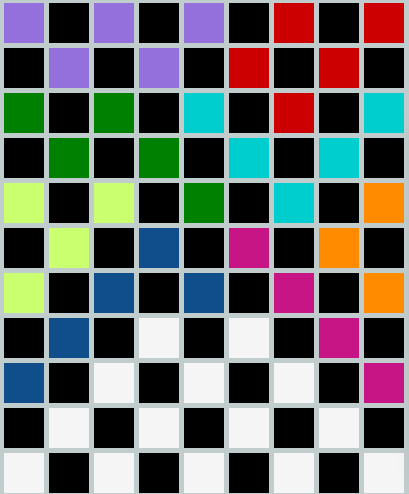
\includegraphics[scale=0.3]{immagini/lv0}
	\caption{Livello 0}
	\label{lev0}
\end{figure}

\subsection{Livello 1}
La configurazione iniziale del livello 1 è mostrata in figura \ref{lev1}. Le forme mancanti da inserire sono mostrate nelle figure \ref{z}, \ref{c}, \ref{y}, \ref{w}.
\begin{figure}[h]
	\centering
	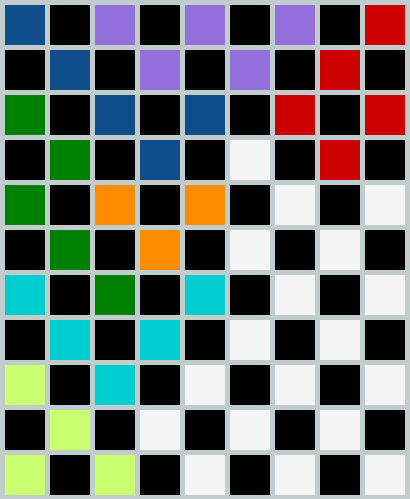
\includegraphics[scale=0.3]{immagini/lv1}
	\caption{Livello 1}
	\label{lev1}
\end{figure}

\subsection{Livello 2}
La configurazione iniziale del livello 2 è mostrata in figura \ref{lev2}. Le forme mancanti da inserire sono mostrate nelle figure \ref{p}, \ref{smallv}, \ref{bigz}, \ref{i}, \ref{w}, \ref{v}.
\begin{figure}[h]
	\centering
	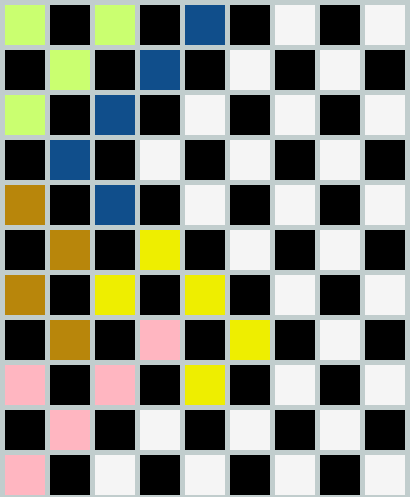
\includegraphics[scale=0.3]{immagini/lv2}
	\caption{Livello 2}
	\label{lev2}
\end{figure}

\subsection{Livello 3}
La configurazione iniziale del livello 3 è mostrata in figura \ref{lev3}. Le forme mancanti da inserire sono mostrate nelle figure \ref{z}, \ref{smallv}, \ref{bigz}, \ref{c}, \ref{y}, \ref{t}, \ref{w}, \ref{v}.
\begin{figure}[h]
	\centering
	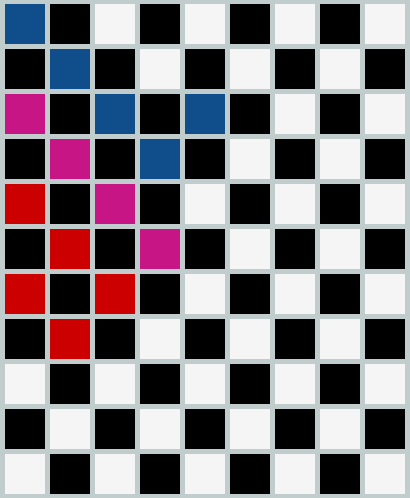
\includegraphics[scale=0.3]{immagini/lv3}
	\caption{Livello 3}
	\label{lev3}
\end{figure}

\subsection{Livello 4}
La configurazione iniziale del livello 4 è mostrata in figura \ref{lev4}. Tutte le forme devono essere inserite nella griglia.
\begin{figure}[h]
	\centering
	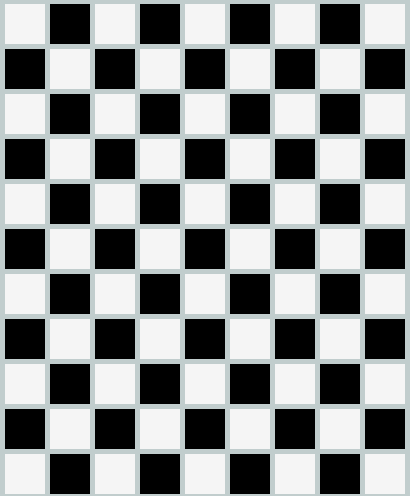
\includegraphics[scale=0.3]{immagini/lv4}
	\caption{Livello 4}
	\label{lev4}
\end{figure}


\section{Possibili miglioramenti}